\section{Polytomous response models}\label{sec:logist-poly}

When the response, $y$, takes on $m > 2$ discrete values, there are
several ways to model the response probabilities.  Let \(\pi_{ij} \equiv
\pi_j \,  ( \vec{x}_i )\) be the probability of response j for case
or group i, given the predictors $\vec{x}_i$.
Because \(\sum_j \,  \pi_{ij} = 1\), only \(m - 1\) of
these probabilities are independent.

The simplest approach uses
the 
\glossterm{proportional odds model}, described in \secref{sec:ordinal}.
This model applies only when the response is ordinal,
\emph{and} an additional assumption
(the proportional odds assumption) holds.  
However, if the
response is purely nominal (e.g., vote Tory, Liberal, Reform, NDP),
or if the proportional odds assumption is untenable, another particularly
simple strategy is to fit separate models to a set of \(m - 1\)
\glossterm{nested dichotomies} derived from the polytomous response
(\secref{sec:nested}).
Both of these methods are handled by \PROC{LOGISTIC}.

A third strategy, described in \secref{sec:genlogit}, is to choose one
    response category (the last, say) as the ``base category'', and
    model the \glossterm{generalized logits} for each of categories
    \(j = 1, 2, \dots , (m - 1)\) compared to category m.  For a
    3-category response, e.g., there are 2 generalized logits,
     \(\logit_{i1}  = \log  ( { \pi_{i1} } /  { \pi_{i3} })\) and
     \(\logit_{i1}  = \log  ( { \pi_{i2} } /  { \pi_{i3} })\).
     These models can be fit using \PROC{CATMOD}.

\section{Models for ordinal variables}\label{sec:loglin-ordinal}
Standard \loglin\ models treat all classification variables as
nominal, unordered factors;
all statistical tests are identical
and parameter estimates are equivalent
if the categories of any variable are reordered.
Yet we have seen that the ordering of categories often provides
important information about the nature of associations
and we showed (\secref{sec:ordinaltests}) that non-parametric
tests which take into account the ordered nature of a factor
are more powerful.

In a mosaic display, an ordered associative effect is seen when
the residuals have an opposite-corner pattern of positive and negative
signs and magnitudes (e.g., for the hair-eye color data,
\figref{fig:mosaic34} or the Titanic data, \figref{fig:mostitanic1}).
In a correspondence analysis plot,
an association has an ordered effect when the points for two factors are
ordered similarly.
In these cases \loglin\ and logit models which use the ordered nature of the factors
offer several advantages.
\begin{itemize}
\item Because they are more focused, tests which use the ordinal
structure of the table variables are more powerful when the association
varies systematically with the ordered values of a factor.

\item Because they consume fewer degrees of freedom,
we can fit unsaturated models where the corresponding model for
nominal factors would be saturated.
In a two-way table, for example, a variety of models for ordinal
factors may be proposed which are intermediate between the independence
model and the saturated model.

\item Parameter estimates from these models are fewer in number, and are
easier to interpret, and quantify the nature of effects better
than corresponding quantities in models for nominal factors.
Estimating fewer parameters typically gives smaller standard errors,
as we saw in \exref{ex:reagan}.
\end{itemize}
These advantages are analogous to the use of tests for trends or
polynomial effects in ANOVA models.

Models for ordinal variables may be specified in \loglin\ form,
as described in \secref{sec:loglin-ordlog}.  When there is an ordinal
response variable, related models may be specified in terms of
logits for adjacent categories (\secref{sec:loglin-ordadj}),
or cumulative logits (\secref{sec:loglin-ordcum}).
The descriptions here are brief. For further information refer to
\citet{Agresti:84}, \citet[Ch. 9]{Agresti:90} and
\citet{Goodman:79,Goodman:83}.

\subsection{Loglinear models for ordinal variables}\label{sec:loglin-ordlog}
For a two-way table, when either the row variable or the column variable,
or both, are ordinal, one simplification comes from assigning ordered
scores, $\{a_i\}, a_1 \le a_2 \le \cdots a_I$, and/or
$\{b_j\}, b_1 \le b_2 \le \cdots b_J$
to the categories
so that the ordinal relations are necessarily included in the model.
Typically, equally spaced scores are used, for example, integer
scores, $\{a_i\}=i$, or the zero-sum equivalent, $\{a_i\}=i-(I+1)/2$
(e.g., $\{a_i\}= \{-1, 0, 1\}$ for $I=3$).
These give simple interpretations of the
association parameters in terms of \emph{local odds ratios},
\begin{equation*}
 \theta_{ij} =
 \frac{ m_{ij} \: m_{i+1, j+1} } { m_{i,j+1} \: m_{i+1, j} }
 \comma
\end{equation*}
the odds ratio for adjacent rows and adjacent columns.

When both variables are assigned scores, we have the \glossterm{linear-by-linear model},
\begin{equation}\label{eq:linlin}
\log ( m_{ij} ) = \mu  +  \lambda_i^A
+  \lambda_j^B  +  \gamma \: a_i b_j \period
\end{equation}
Because the scores are fixed, this model has only one extra parameter, $\gamma$, compared to the
independence model, which is the special case, $\gamma=0$.
The terms  $\gamma a_i b_j $ describe a pattern of association
where deviations from independence increase linearly with $a_i$
and $b_j$ in opposite directions towards the opposite corners of
the table.

In the linear-by-linear association model, the local log odds ratios
are
\begin{equation*}
\log \theta_{ij} =
 \gamma (a_{i+1} - a_i) (b_{j+1} - b_j)
 \comma
\end{equation*}
which reduces to
\begin{equation*}
\log \theta_{ij} =
 \gamma
\end{equation*}
for integer-spaced scores, so $\gamma$ is the common local log odds ratio.
As a result, the linear-by-linear model is sometimes called the
model of \emph{uniform association} \citep{Goodman:79}.
\ix{uniform association model}
\ix{linear-by-linear model}
\ix{log odds ratio!local}

Generalizations of the linear-by-linear model result when only one
variable is assigned scores.
In the \glossterm{row-effects model},
the row variable, say, $A$ is treated as nominal, while
the column variable, $B$, is assigned ordered scores $\{b_j\}$.
The \loglin\ model is then
\begin{equation}\label{eq:roweff}
 \log ( m_{ij} ) = \mu  +  \lambda_i^A
  +  \lambda_j^B  +  \alpha_i b_j
 \comma
\end{equation}
where the $\alpha_i$ parameters are the \emph{row effects}.
An additional constraint,
$\sum_i \alpha_i =0$ or $\alpha_I =0$
 is imposed, so that model \eqref{eq:roweff}
has $(I-1)$ more parameters than the independence model.
The linear-by-linear model is the special case where the row effects
are equally spaced, and the independence model is the special case
where all $\alpha_i = 0$.

The row-effects model \eqref{eq:roweff} also has a simple odds ratio interpretation.
The local log odds ratio for adjacent pairs of rows and columns is
\begin{equation*}
\log \theta_{ij} =
  \alpha_{i+1} - \alpha_i
  \comma
\end{equation*}
which is constant for all pairs of adjacent columns.  Plots of the
local log odds ratio against $i$ would appear as a set of parallel
curves.

In the analogous \glossterm{column-effects model}, $(J-1)$ linearly independent
column effect
parameters $\beta_j$ are estimated for the column variable, while fixed
scores $\{a_i\}$ are assigned to the row variable.

The linear-by-linear model \eqref{eq:linlin} and the row-effects model
\eqref{eq:roweff} can be fit using \PROC{CATMOD},
but to do so requires that you enter the complete model matrix explicitly.
With \PROC{GENMOD} you need only create a numeric variable with score
values in the input \Dset, a much easier task.
\begin{Example}[mental2]{Mental impairment and parents' SES}
In \exref{ex:mental1} \CA\ was used to explore the relationship between
ratings of the mental health status of young New Yorkers and
their parents' socioeconomic status (SES).
\figref{fig:correses} showed that most of the association in the
table was accounted for by a single dimension along which both factors
were ordered, consistent with the view that mental health increased
in relation to parents' SES.

For comparison, we first fit the independence model with both
\PROC{CATMOD} and \PROC{GENMOD}.
As we expect, this model fits quite badly,
with $\GSQ\ (15) = 47.418$.
\begin{listing}
%include catdata(mental);
proc catmod data=mental;
   weight count;
   model mental*ses = _response_ / noiter noprofile noresponse;
   loglin mental ses / title='Independence';
   run;
\end{listing}
For illustration, the standardized (adjusted) deviance residuals,
$g_i / \sqrt ( 1 - h_i )$
are obtained in the \PROC{GENMOD}
step (named \pname{stresdev} in the \pname{obstats} \Dset),
and used with the \macro{MOSAIC} to produce the mosaic
display shown in the left panel of \figref{fig:mental2}.%
\footnote{To ensure that the the levels of both factors are ordered
correctly, \pname{MENTAL} and \pname{SES} were entered as numeric
variables in the \Dset\ \pname{MENTAL}, and user-formats were used
to provide the character labels shown in \figref{fig:mental2}.
Because \IML\ does not make use of formatted values, the \macro{TABLE}
was used to convert the numeric variables to character.
}
The parameter \pname{cellfill=dev 0.5}
causes the program to write the value of all residuals greater than 0.5
in absolute value in the corresponding tile.
\begin{listing}
proc genmod data=mental;
   class mental ses;
   model count = mental ses / dist=poisson obstats residuals;
   make 'obstats' out=obstats noprint;
run;

%table(data=mental, var=Mental SES, weight=count, char=Y,
       format=mental mental. ses ses., order=data, out=mental2);
data obstats;
   merge mental2 obstats;
%mosaic(data=obstats, vorder=Mental SES, plots=2, split=H V, resid=stresdev,
   title=Mental Impairment and SES: Independence, cellfill=dev 0.5);
\end{listing}
%% two subfig side-by-side
\begin{figure}[htb]
 \begin{minipage}[t]{.49\linewidth}
  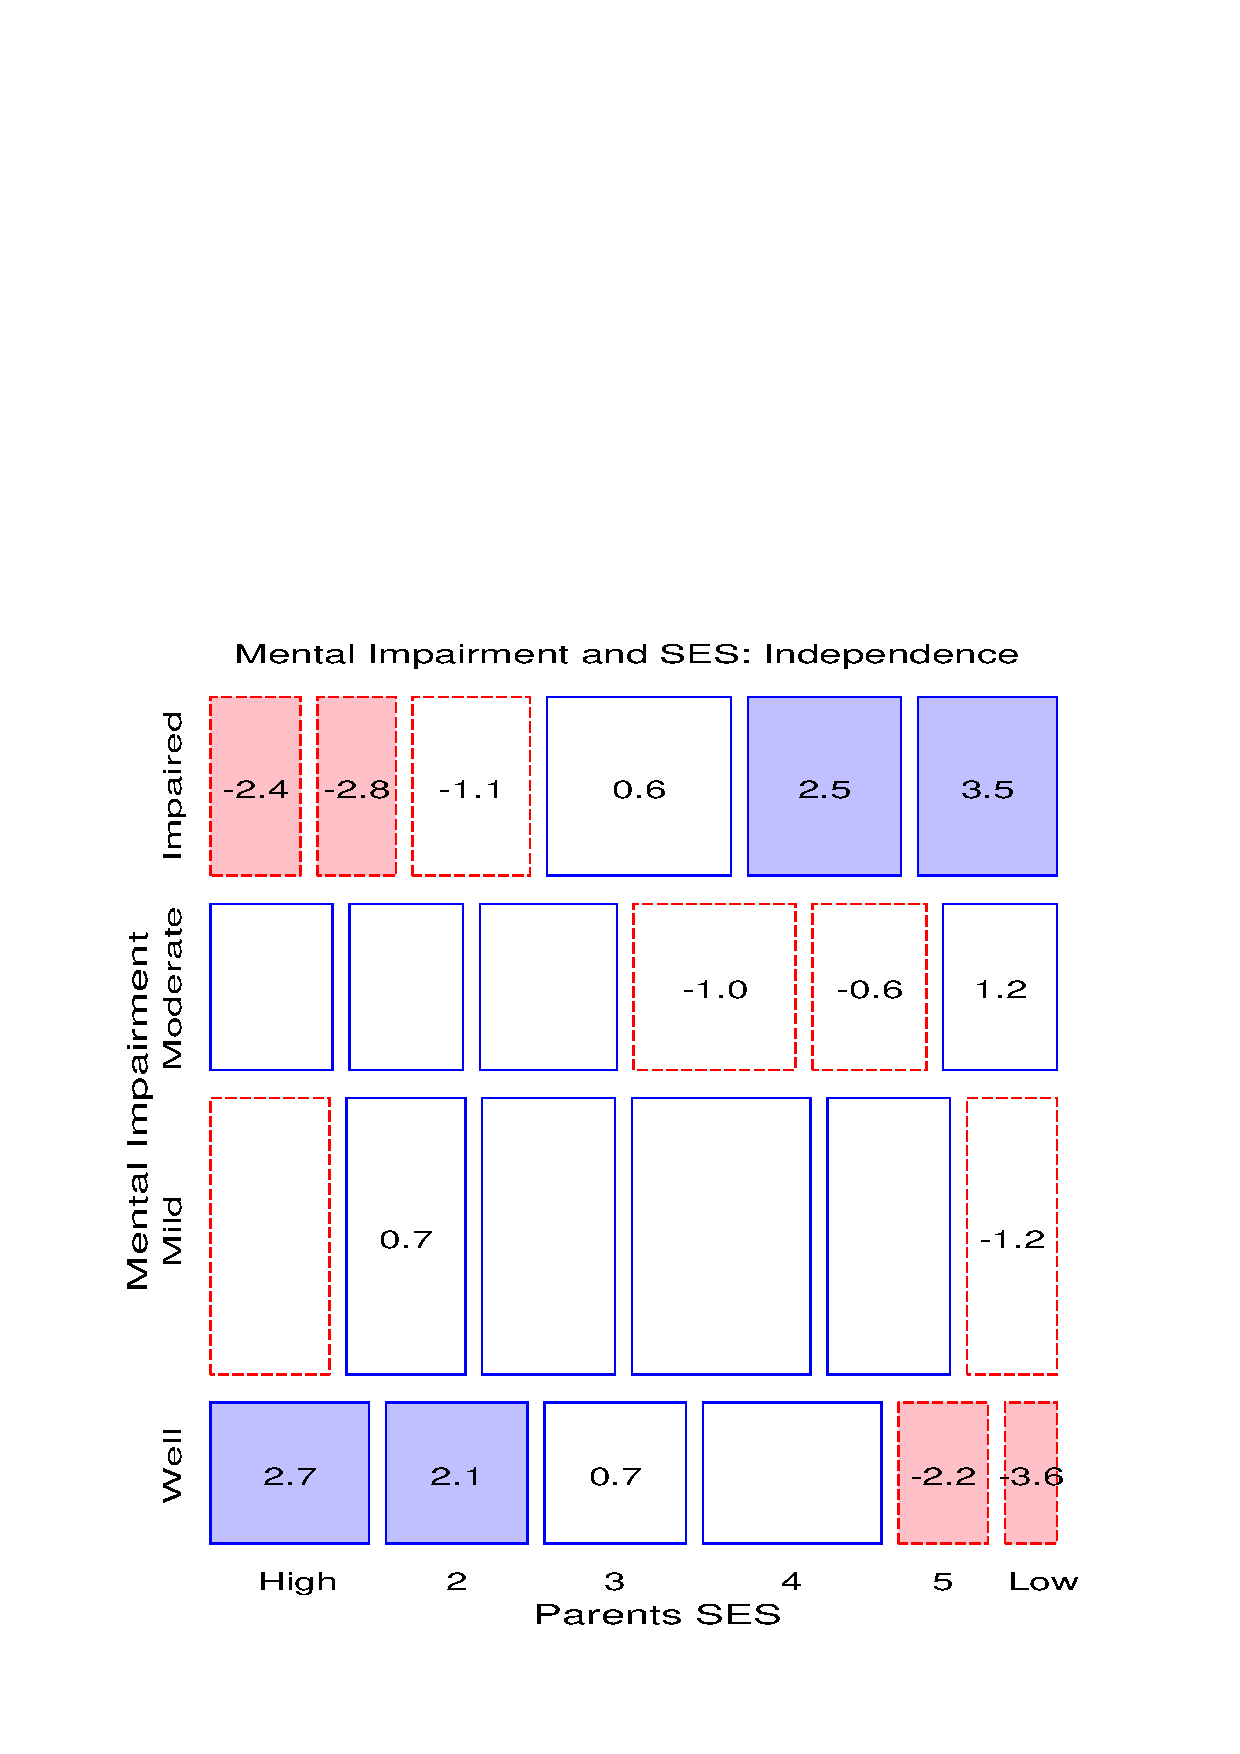
\includegraphics[width=1\linewidth]{mental21}
 \end{minipage}%
 \hfill
 \begin{minipage}[t]{.49\linewidth}
  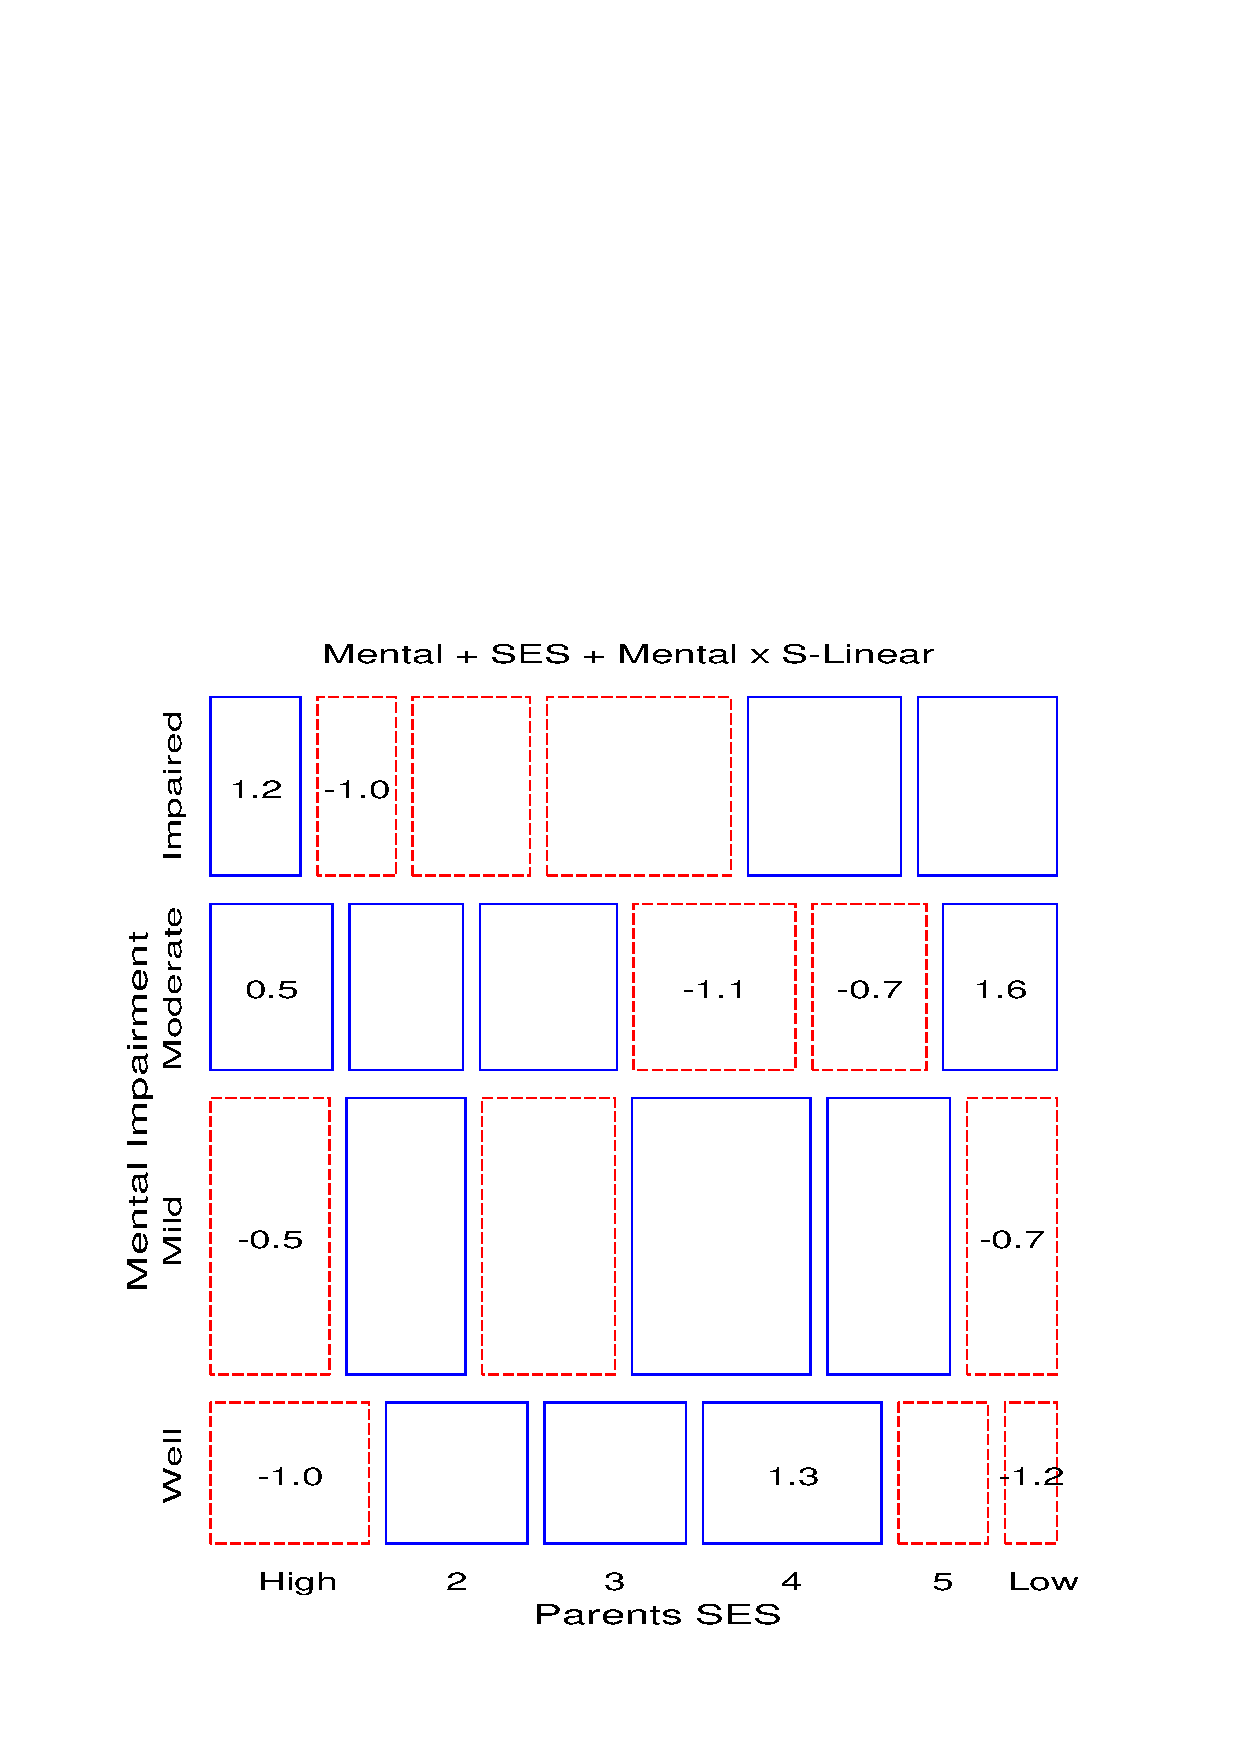
\includegraphics[width=1\linewidth]{mental22}
 \end{minipage}
 \caption[Mental health and SES: Residuals]{Mental health and SES: Residuals from Independence (left) and Row Effects (right) Models}\label{fig:mental2}
\end{figure}
Note that the residuals in \figref{fig:mental2} for the
independence model have the opposite-corner pattern which would
arise if either the row-effects model (with ordered row effects)
or the linear-by-linear
association model described the association between mental health
and SES.
\begin{table}[htb]
 \caption{Mental health data: Goodness-of-fit statistics for ordinal \loglin\ models}\label{tab:mentab2}
 \begin{center}
 \begin{tabular}{l rrrr r}
  \hline
  Model                & df & $\chisq$ & $\GSQ$ & $\Delta \GSQ$  & AIC \\ 
  \hline
  Independence         & 15 & 45.985 & 47.418 & .    &  17.42\\ 
  Linear-by-linear     & 14 & 9.732 & 9.895 & 37.523 & -18.18\\ 
  Row-effects (Mental) & 12 & 6.289 & 6.281 & 41.137 & -17.72\\ 
  \hline
 \end{tabular}
 \end{center}
\end{table}



To fit models in which the association terms for \pname{mental} and/or
\pname{ses} use quantitative scores, create copies, \pname{M} and
\pname{S} of these variables.  They are used as quantitative variables
when they appear in the \stmt{MODEL}{GENMOD}, but are \emph{not} listed
as \pname{CLASS} variables.
The following statements fit the row-effects model, using SES
as a linear effect, and then the linear-by-linear model.
Goodness-of-fit statistics for all three models are shown in
\tabref{tab:mentab2}.

\begin{listing}
data mental;
   set mental;
   m = mental;    *-- copy m and s as quantitative, non-class;
   s = ses;

title 'Linear SES';
proc genmod data=mental;
   class mental ses;
   model count = mental ses mental*s / dist=poisson obstats residuals;
   make 'obstats' out=obstats noprint;
run;
data obstats;
   merge mental obstats;
%mosaic(data=obstats, var=Mental SES, resid=stresdev,  split=H V,
   title=Mental + SES + Mental x S-Linear, cellfill=dev 0.5);

title 'Linear x Linear';
proc genmod data=mental;
   class mental ses;
   model count = mental ses m*s / dist=poisson obstats residuals;
run;
\end{listing}
The $\Delta \GSQ$ values in \tabref{tab:mentab2} each test whether
the corresponding model results in a significant reduction in the
residual $\GSQ$ compared to the independence model.  Both are
highly significant.

Similarly, the difference in $\GSQ$ between the linear-by-linear
and row-effects model, $\Delta \GSQ\ (2) = 9.732-6.289 = 3.443$ suggests that the 
row-effects model
is \emph{not} a significant improvement over the
linear-by-linear model.
The AIC values suggest a slight preference for the linear-by-linear model.
The residuals for the row effects model are shown in the right
panel of \figref{fig:mental2}; residuals for the linear-by-linear
model (not shown) have the same signs, but are slightly smaller
in some cells.

\begin{Output}[htb]
\caption{Parameter estimates for the row-effects \loglin\ model, Mental health data}\label{out:mental2.1}
\small
\verbatiminput{ch7/out/mental2.1}
\end{Output}

Under the linear-by-linear model, the estimate of the coefficient of
\pname{M*S} is $\hat{\gamma} = 0.0907$ (s.e.=0.015) with unit-spaced scores.
This corresponds to a local odds ratio, $\hat{\theta}_{ij} = \exp (0.0907) = 1.095$.
This single number describes the association succinctly:
each step down socioeconomic scale increases the odds of being classified
one step poorer in mental health by 9.5\%.

Parameter estimates for the row-effects model are shown in
\outref{out:mental2.1}.  The row effects are the values of
the \pname{S*MENTAL} terms.  These values are ordered, consistent with
mental health status having ordinal associative effects,
but (with integer scores for both variables) they are not equally
spaced, as the linear-by-linear model would imply.
The spacing of these parameter estimates is similar to what we saw
in the \CA\ plot (\figref{fig:correses}), with the middle categories
Mild Impairment, and Moderate Impairment relatively close together
compared to the extreme categories.

These \loglin\ models and the associated mosaic displays do not
provide a clear preference between the row-effects and linear-by-linear
models here.
We turn now to other models and graphical displays which may distinguish them better.
\end{Example}


\subsection{Adjacent category logit models}\label{sec:loglin-ordadj}
When there is a single response variable, logit models provide a
simple way to model the dependence of the response on the other,
explanatory variables.  For an ordinal response,
models for the logits between adjacent response categories
allow the ordered nature of the response to be taken into account.
For the model of independence, the \emph{adjacent category logits} are
\begin{eqnarray}
A_{j| i} \equiv
\log \left(
 \frac{ \pi_{j+1|i} } { \pi_{j|i} }
 \right) =
\log \left(
 \frac{ m_{i, j+1} } { m_{ij} }
 \right)
  & = &
( \mu  +  \lambda_i^A +  \lambda_{j+1}^B ) -
( \mu  +  \lambda_i^A +  \lambda_j^B )  \nonumber \\
  & = &  \lambda_{j+1}^B -  \lambda_{j}^B \label{eq:aindep}
\end{eqnarray}
which are constants, say, $\beta_j = (\lambda_{j+1}^B -  \lambda_{j}^B )$
not depending on the explanatory variable(s).
If an explanatory variable is also ordinal, we may use scores, $\{a_i\}$
as before.
The analog of the linear-by-linear model with unit-spaced scores
allows the value of $A_{j| i}$ to vary linearly with the quantitative value,
\begin{equation}\label{eq:alin}
A_{j| i} = \beta_j + \gamma \: a_i
\end{equation}
The slope parameter $\gamma$ has a similar log odds interpretation:
the log odds of a response in category $j+1$
as opposed to category $j$ increases by $\gamma$
for each unit increase in the explanatory variable.
% The intercept parameters, $\beta_j$ ...

In a similar way, the fixed scores $a_i$ may be replaced by row effect
parameters, $\alpha_i$ to be estimated (with the constraint $\sum_i \alpha_i =0$ or $\alpha_I =0$)
to give the row-effects adjacent logit model
\begin{equation}\label{eq:arow}
A_{j| i} = \beta_j + \alpha_i
\end{equation}
A plot of the fitted logits against $i$ for this model appears as parallel
curves (rather than parallel lines under the linear-by-linear model
\eqref{eq:alin}).

Even less restrictive models, which are still unsaturated, may be fit if the row-effects model fits poorly.  For example, each adjacent logit may be
linearly related to an assigned score for an explanatory variable,
but the slopes may differ over the adjacent response categories
(the \emph{linear-interaction model}):
\begin{equation}\label{eq:alin-int}
A_{j| i} = \beta_j + \gamma_j \: s_i \period
\end{equation}
Alternatively, a quadratic relation between the
adjacent logits, $A_{j| i}$ and the scores,
$A_{j| i} = \beta_j + \gamma_1 \: a_i + \gamma_2 a_i^2$
may be fit.
These possibilities are illustrated below.

\begin{Example}[mental4]{Mental impairment and parents' SES}
We consider here adjacent category logit models for the Mental Health
data, treating \pname{MENTAL} as an ordinal response.
Adjacent logit models are easily fit with \PROC{CATMOD}
using the \pname{RESPONSE ALOGIT;} statement.
Differences among the logits for adjacent categories (the intercepts, $\beta_j$, in models \eqref{eq:alin} and \eqref{eq:arow}) are
specified by the \verb|_RESPONSE_| keyword in the
\stmt{MODEL}{CATMOD}.  Nominal explanatory variables are included
as main effects (and possibly, interactions) on the left-hand side
of the \stmt{MODEL}{CATMOD}.  An explanatory variable is treated
as quantitative when declared in a \stmt{DIRECT}{CATMOD}.

The following statements fit a series of adjacent category logit models
to the Mental Health data.  Model 0 has only a \verb|_RESPONSE_|
effect, and is analogous to the independence model.
In Model 1, the adjacent logits for mental impairment are affected
by SES, as a nominal variable.
Model 2 is the linear-by-linear model for adjacent logits, with
SES as a direct variable,
while Model 3 allows different slopes for each adjacent logit.
%% input: /users/faculty/friendly/sasuser/catdata/mental4.sas
%% last modified: 01-Dec-98 12:07
\begin{listing}
%include catdata(mental);

*-- Adjacent logit models;
proc catmod data=mental;
   weight count;
   population ses;
   response alogit / out=pred0;
   model mental = _response_ / noprofile noresponse title='Model 0:  _R_';
  run;
   response alogit / out=pred1;
   model mental = _response_  ses / noprofile noresponse title='Model 1: _R_ SES';
  run;
   direct ses;
   response alogit / out=pred2;
   model mental = _response_  ses / noprofile noresponse title='Model 2: _R_ S';
  run;
   direct ses;
   response alogit / out=pred3;
   model mental = _response_ | ses / noprofile noresponse title='Model 3: _R_|S';
  run;
\end{listing}

%% two subfig side-by-side
\begin{figure}[htb]
 \begin{minipage}[t]{.49\linewidth}
  \includegraphics[width=1\linewidth]{mental41}
 \end{minipage}%
 \hfill
 \begin{minipage}[t]{.49\linewidth}
  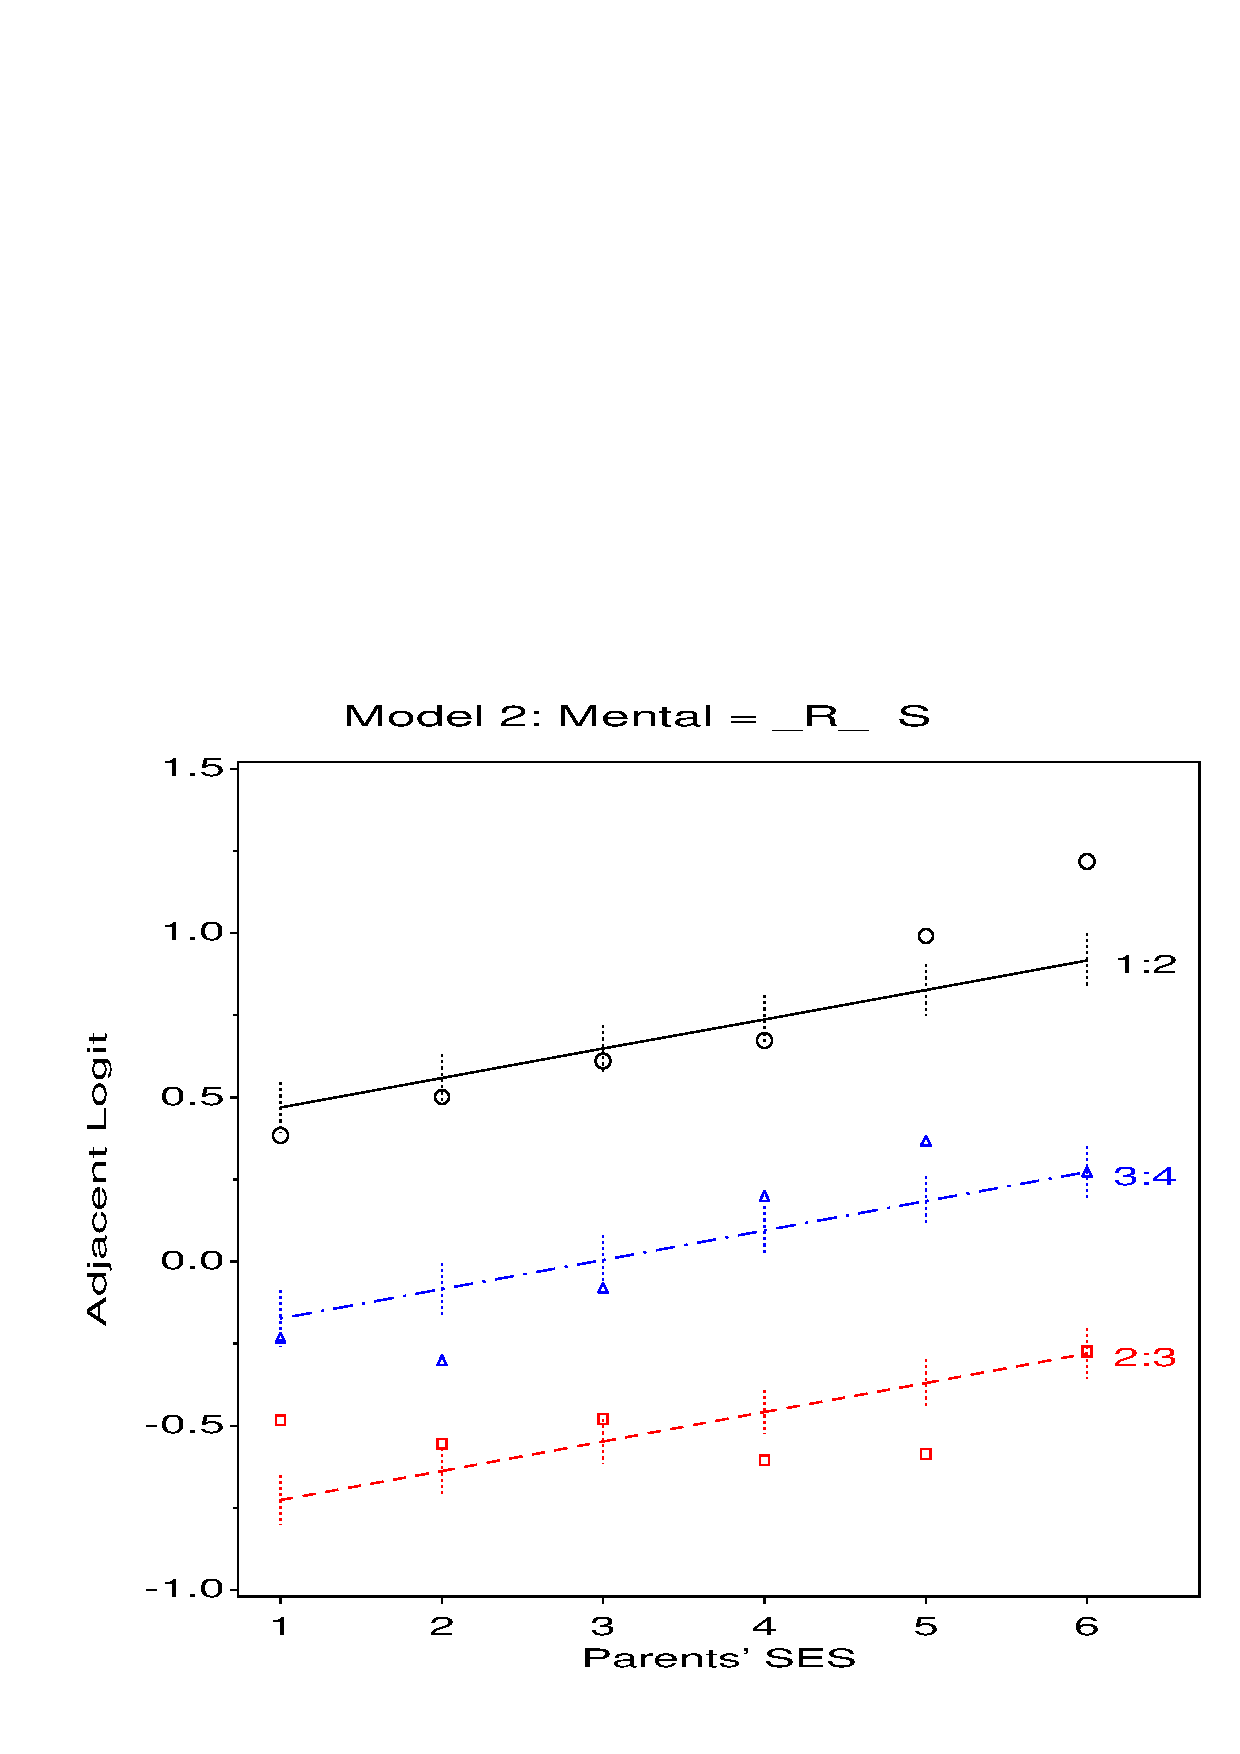
\includegraphics[width=1\linewidth]{mental42}
 \end{minipage}
 \caption{Adjacent category logit models for Mental Health data, Model 1 and Model 2}\label{fig:mental4a}
\end{figure}
\begin{table}[htb]
 \caption{Adjacent category logit models for Mental Health data}\label{tab:mentab4}
 \begin{center}
 \renewcommand{\arraystretch}{1.1}
 \begin{tabular}{c ll rrr r}
  \hline
  Model & Formula & Terms & df & \chisq\ & $p$-value & AIC\\ 
  \hline
  0 & $A_{j| i} = \beta_j $                  & \verb\_R_\     & 15 & 44.35 & 0.0001 & 14.35\\ 
  1 & $A_{j| i} = \beta_j + \alpha_i$        & \verb\_R_ SES\ & 10 & 6.76 & 0.7478  & -13.24\\ 
  2 & $A_{j| i} = \beta_j + \gamma \: a_i$   & \verb\_R_ S\   & 14 & 9.68 & 0.7849  & -18.32\\ 
  3 & $A_{j| i} = \beta_j + \gamma_j a_i$    & \verb\_R_|S\   & 12 & 6.26 & 0.9023 & -17.74\\ 
  4 & $A_{j| i} = \beta_j + \gamma_1 a_i + \gamma_2 a_i^2$ & \verb\_R_ S S^2\ & 13 & 7.39 & 0.8809 & -18.61\\ 
  5 & $A_{j| i} = \beta_j + \gamma_j a_i + \delta a_i^2$ & \verb\_R_|S S^2\ & 11 & 3.69 & 0.9782 & -18.69\\ 
  \hline
 \end{tabular}
 \end{center}
\end{table}

For each model, an \ODS, which contains the observed and fitted logits,
is requested with the \opt{OUT=}{CATMOD} in the \stmt{RESPONSE}{CATMOD}.
Plotting the observed and fitted logits
makes it easy to see what relationships are implied by each model.
The plots for Model 1 and Model 2, shown in \figref{fig:mental4a},
are produced with the \macro{CATPLOT}
as shown below.
The macro call requests a plot of the observed logit
(\verb|_OBS_|) against \pname{SES}, with separate curves for each
adjacent logit (\verb|CLASS=_NUMBER_|).
By default, the macro also draws curves connecting the predicted
values (\verb|_PRED_| in the \ODS) and $\pm 1$ standard error bars
around each fitted logit.
\begin{listing}
axis1 label=(a=90) order=(-1 to 1.5 by .5);
axis2 offset=(3,8);
proc format;
   value cum 1='1:2'  2='2:3'  3='3:4';
title 'Model 1: Mental = _R_ SES';
%catplot(data=pred1, x=ses, y=_obs_, class=_number_, clfmt=cum.,
   type=FUNCTION, ylab=Adjacent Logit);

title 'Model 2: Mental = _R_  S';
%catplot(data=pred2, x=ses, y=_obs_, class=_number_, clfmt=cum.,
   type=FUNCTION, ylab=Adjacent Logit);
\end{listing}

For illustration, we also fit less restrictive models,
allowing a quadratic relation between the adjacent logit and SES (Model 4).
Model 5 adds a quadratic term
to the unequal slopes allowed in Model 3.
Plots for Model 3 and Model 5 are shown in \figref{fig:mental4b}.
%% input: /Users/friendly/sasuser/catdata/mental4.sas
%% last modified: 19-Aug-99 11:31
\begin{listing}
proc catmod data=mental;
   weight count;
   population ses;
   direct ses;
   response alogit / out=pred4;
   model mental = _response_ ses ses*ses / noprofile noiter title='Model 4: _R_ S S^2';
  run;
   response alogit / out=pred5;
   model mental = _response_|ses ses*ses / noprofile noiter title='Model 5: _R_|S S^2';
  run;
\end{listing}


%% two subfig side-by-side
\begin{figure}[htb]
 \begin{minipage}[t]{.49\linewidth}
  \includegraphics[width=1\linewidth]{mental43}
 \end{minipage}%
 \hfill
 \begin{minipage}[t]{.49\linewidth}
  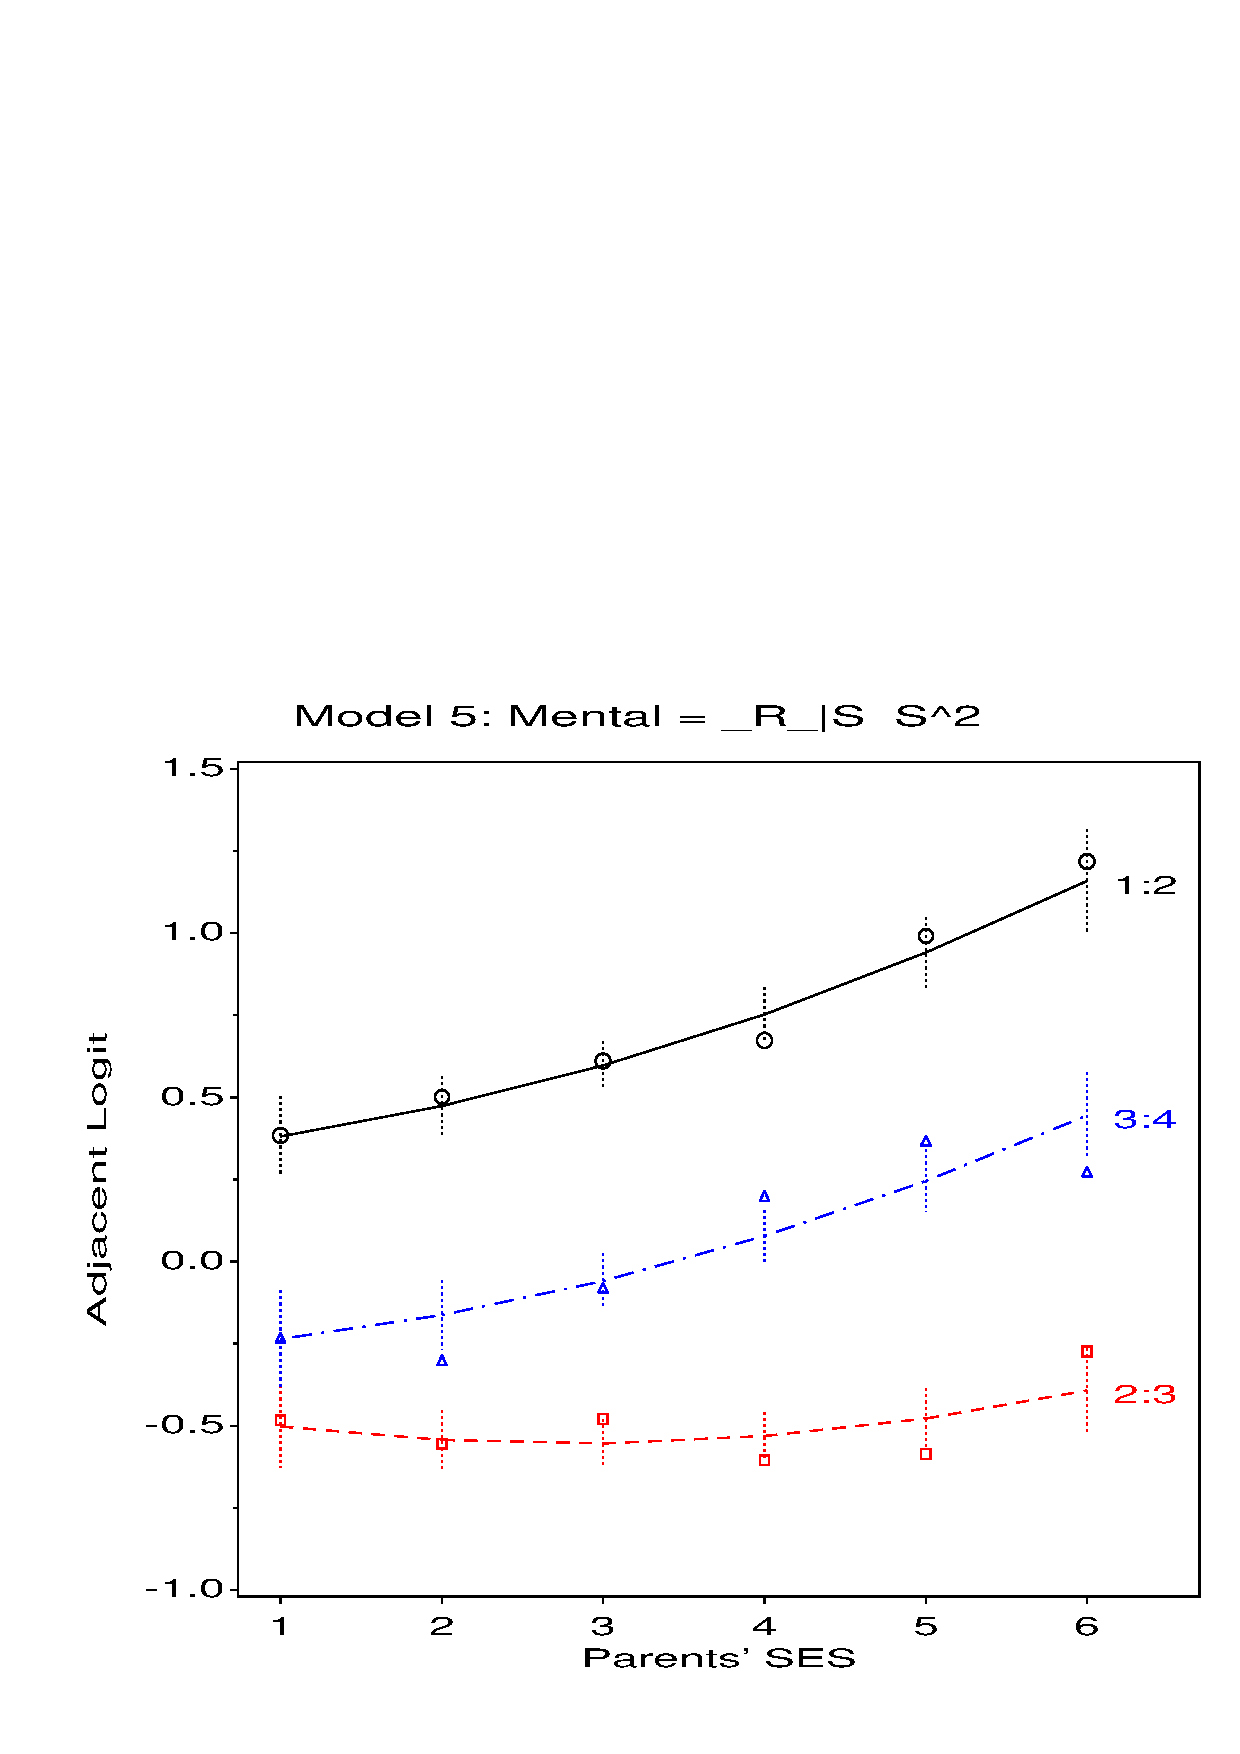
\includegraphics[width=1\linewidth]{mental44}
 \end{minipage}
 \caption{Adjacent category logit models for Mental Health data: Model 3 and Model 5}\label{fig:mental4b}
\end{figure}

What may we conclude from this?
From \tabref{tab:mentab4}, all models except the independence model
have acceptable fit according to the \chisq\ values;
Models 2--5 all have smaller AIC values than Model 1;  of these,
Model 2, the linear-by-linear is the most parsimonious, but Models
4 and 5 have slightly smaller AIC values.

One interpretation, from the plots in \figref{fig:mental4a} and \figref{fig:mental4b}
is that there is evidence that not both of SES and mental impairment
can be considered linear with unit spacing.
The intercepts suggest that the gap between categories 1 and 2
(`Well', 'Mild impairment') is greatest on the mental health scale,
and that between categories 2 and 3 (`Mild', `Moderate impairment')
is smallest.
The evidence regarding the metric for SES is more ambiguous:
there is a suggestion of a mildly quadratic relationship with SES,
particularly for the logit between response categories 1 and 2,
but this may be due to the points for (lowest) SES categories 5 and 6,
where the large logit values imply
a relatively larger number of people
classified as mildly impaired as opposed to well.
\end{Example}


\subsection{Cumulative logit models}\label{sec:loglin-ordcum}
When there is an ordinal response factor, cumulative logit models
\citep{WilliamsGrizzle:72} provide
an alternative way to take the ordinal nature of the response into account,
without assigning arbitrary scores to the response categories.

Let $F_j$ be the cumulative probability of a response less than or equal
to category $j$,
\begin{equation*}
F_j = \pi_1 + \pi_2 + \cdots + \pi_j  = \sum_{h=1}^{h=j} \pi_h
 \period
\end{equation*}
Then the \emph{cumulative logit} is defined as
\begin{equation*}%\label{eq:cumlogit}
C_j \equiv \logit ( 1 - F_j ) =
  \log \left( \frac { 1 - F_j }{F_j} \right) \period
\end{equation*}
$C_j$ gives the log odds that the response is in a category \emph{greater} than
category $j$, as opposed to a category less than or equal to $j$.
By this definition, the cumulative logits are necessarily
monotone decreasing over the response categories:
$C_1 \ge C_2 \ge \cdots \ge C_{J-1}$.
Models for the cumulative logit are particularly useful when the
response may be considered a discrete realization of an underlying
continuous variable.

In terms of cumulative logits, the model of independence is
\begin{equation*}%\label{eq:cindep}
C_{j|i} = \beta_j \comma
\end{equation*}
that is, the logit does not depend on explanatory variable(s) indexed
by subscript $i$.
Here, the response category parameters $\beta_j$ refer to the
cutpoints between adjacent categories, rather than to the distances
between adjacent ones as in the analogous adjacent category logit
model \eqref{eq:aindep}.

For quantitative scores, $a_i$, assigned to an explanatory variable,
the analog of the linear-by-linear model is
\begin{equation}\label{eq:clin}
 C_{j| i} = \beta_j + \gamma \: a_i
 \period
\end{equation}
which again has one more parameter than the independence model.
For any two rows, the difference in logits,
$C_{j| i} - C_{j| i'}$
is the log odds ratio in the $2\times 2$ table
for those two rows, with columns dichotomized following response category $j$.
Under model \eqref{eq:clin}, $C_{j| i} - C_{j| i'} = \gamma ( a_i - a_{i'})$,
so the log odds ratio is proportional to the difference in scale values,
and is the same at all cutpoints.
When unit-spaced scores, $\{a_i\} = i$ are used, the logit difference for
adjacent rows is then constant:
\begin{equation*}
 C_{j| i} - C_{j| i'} = \gamma
 \period
\end{equation*}

As with the adjacent category logits, a variety of models analogous to
the row effects model \eqref{eq:arow}, and
the linear-interaction model \eqref{eq:alin-int}
may be defined for the cumulative logits.
We illustrate these below, primarily to look at the shapes of plots
of observed and fitted logits, and to compare them with what we saw for
adjacent category logits.
\begin{Example}[mental3]{Mental impairment and parents' SES}
Cumulative logit models may be fit using \PROC{CATMOD} with the
\pname{RESPONSE CLOGIT;} statement.
The model is specified in the same way as for adjacent category
logits, but now the \verb|_RESPONSE_| keyword refers to
differences among the cumulative response probabilities.
As before,
an independent variable is treated as a quantitative variable,
when it is declared in a \stmt{DIRECT}{CATMOD}.

The following statements fit
the same models as in \exref{ex:mental4}: first Models 0--3
in which SES has no effect on mental health (Model 0), then SES with
a nominal effect (Model 1), a constant linear effect (Model 2)
and different linear effects for each cumulative logit (Model 3).
%% input: /users/faculty/friendly/sasuser/catdata/mental3.sas
%% last modified: 26-Nov-98 17:27
\begin{listing}
%include catdata(mental);

*-- Cumulative logit models;
proc catmod data=mental;
   weight count;
   population ses;
   response clogit / out=pred0;
   model mental = _response_ / noprofile noresponse title='Model 0: _R_';
  run;
   response clogit / out=pred1;
   model mental = _response_  ses / noprofile noresponse title='Model 1: _R_ SES';
  run;
   direct ses;
   response clogit / out=pred2;
   model mental = _response_  ses / noprofile noresponse title='Model 2:  _R_ S';
  run;
   direct ses;
   response clogit / out=pred3;
   model mental = _response_ | ses / noprofile noresponse title='Model 3:  _R_|S';
  run;
\end{listing}


For comparison, we also fit models with both linear and quadratic
effects on the cumulative logits,
first with equal slopes and curvature
for all response categories (Model 4), and second with separate slopes and
equal curvatures (Model 5).
%% input: /users/faculty/friendly/sasuser/catdata/mental3.sas
%% last modified: 29-Nov-98 11:55
\begin{listing}
data mental;
   set mental;
   ses2 = ses**2;

proc catmod data=mental;
   weight count;
   population ses;
   direct ses ses2;
   response clogit / out=pred4;
   model mental = _response_ ses ses2 / noprofile noiter title='Model 4: _R_ S S^2';
  run;
   response clogit / out=pred5;
   model mental = _response_|ses ses2 / noprofile noiter title='Model 5: _R_|S S^2';
  run;
\end{listing}


The model fit statistics for these models are shown in \tabref{tab:mentab3}.
The values are quite similar to those for the adjacent category logits
(\tabref{tab:mentab2}).
\begin{table}[htb]
 \caption{Cumulative logit models for Mental Health data}\label{tab:mentab3}
 \begin{center}
 \begin{tabular}{c l rrr r}
  \hline
  Model & Terms        & df & \chisq & $p$-value & AIC\\ 
  \hline
  0 & \verb\_R_\       & 15 & 45.92 & 0.0001 &  15.92\\ 
  1 & \verb\_R_| SES\  & 10 &  7.75 & 0.6536 & -12.25\\ 
  2 & \verb\_R_ S\     & 14 & 10.72 & 0.7080 & -17.28\\ 
  3 & \verb\_R_|S\     & 12 &  6.48 & 0.8897 & -17.52\\ 
  4 & \verb\_R_ S S^2\ & 13 &  8.36 & 0.8192 & -17.64\\ 
  5 & \verb\_R_|S S^2\ & 11 &  3.94 & 0.9716 & -18.06\\ 
  \hline
 \end{tabular}
 \end{center}
\end{table}


For any such model, the \macro{CATPLOT} displays the observed and fitted
cumulative logits using the \ODS\ specified on the
\stmt{RESPONSE}{CATMOD}.
The statements below produce the graphs of the logits for Model 0,
and Model 1,
shown in \figref{fig:mental3a}.
Similar statements, using the \ODS s \pname{PRED2} and \pname{PRED4},
give the graphs for Model 2 and Model 4 in \figref{fig:mental3b}.
%% input: /users/faculty/friendly/sasuser/catdata/mental3.sas
%% last modified: 02-Dec-98 15:47
\begin{listing}
axis1 label=(a=90);
axis2 offset=(3,6);
proc format;
   value cum 1='>1'  2='>2'  3='>3';
title 'Model 0: Mental = _R_';
%catplot(data=pred0, x=ses, y=_obs_, class=_number_, clfmt=cum.,
   type=FUNCTION, ylab=Cumulative Logit);
title 'Model 1: Mental = _R_ SES';
%catplot(data=pred1, x=ses, y=_obs_, class=_number_, clfmt=cum.,
   type=FUNCTION, ylab=Cumulative Logit);
\end{listing}


%% two subfig side-by-side
\begin{figure}[htb]
 \begin{minipage}[t]{.49\linewidth}
  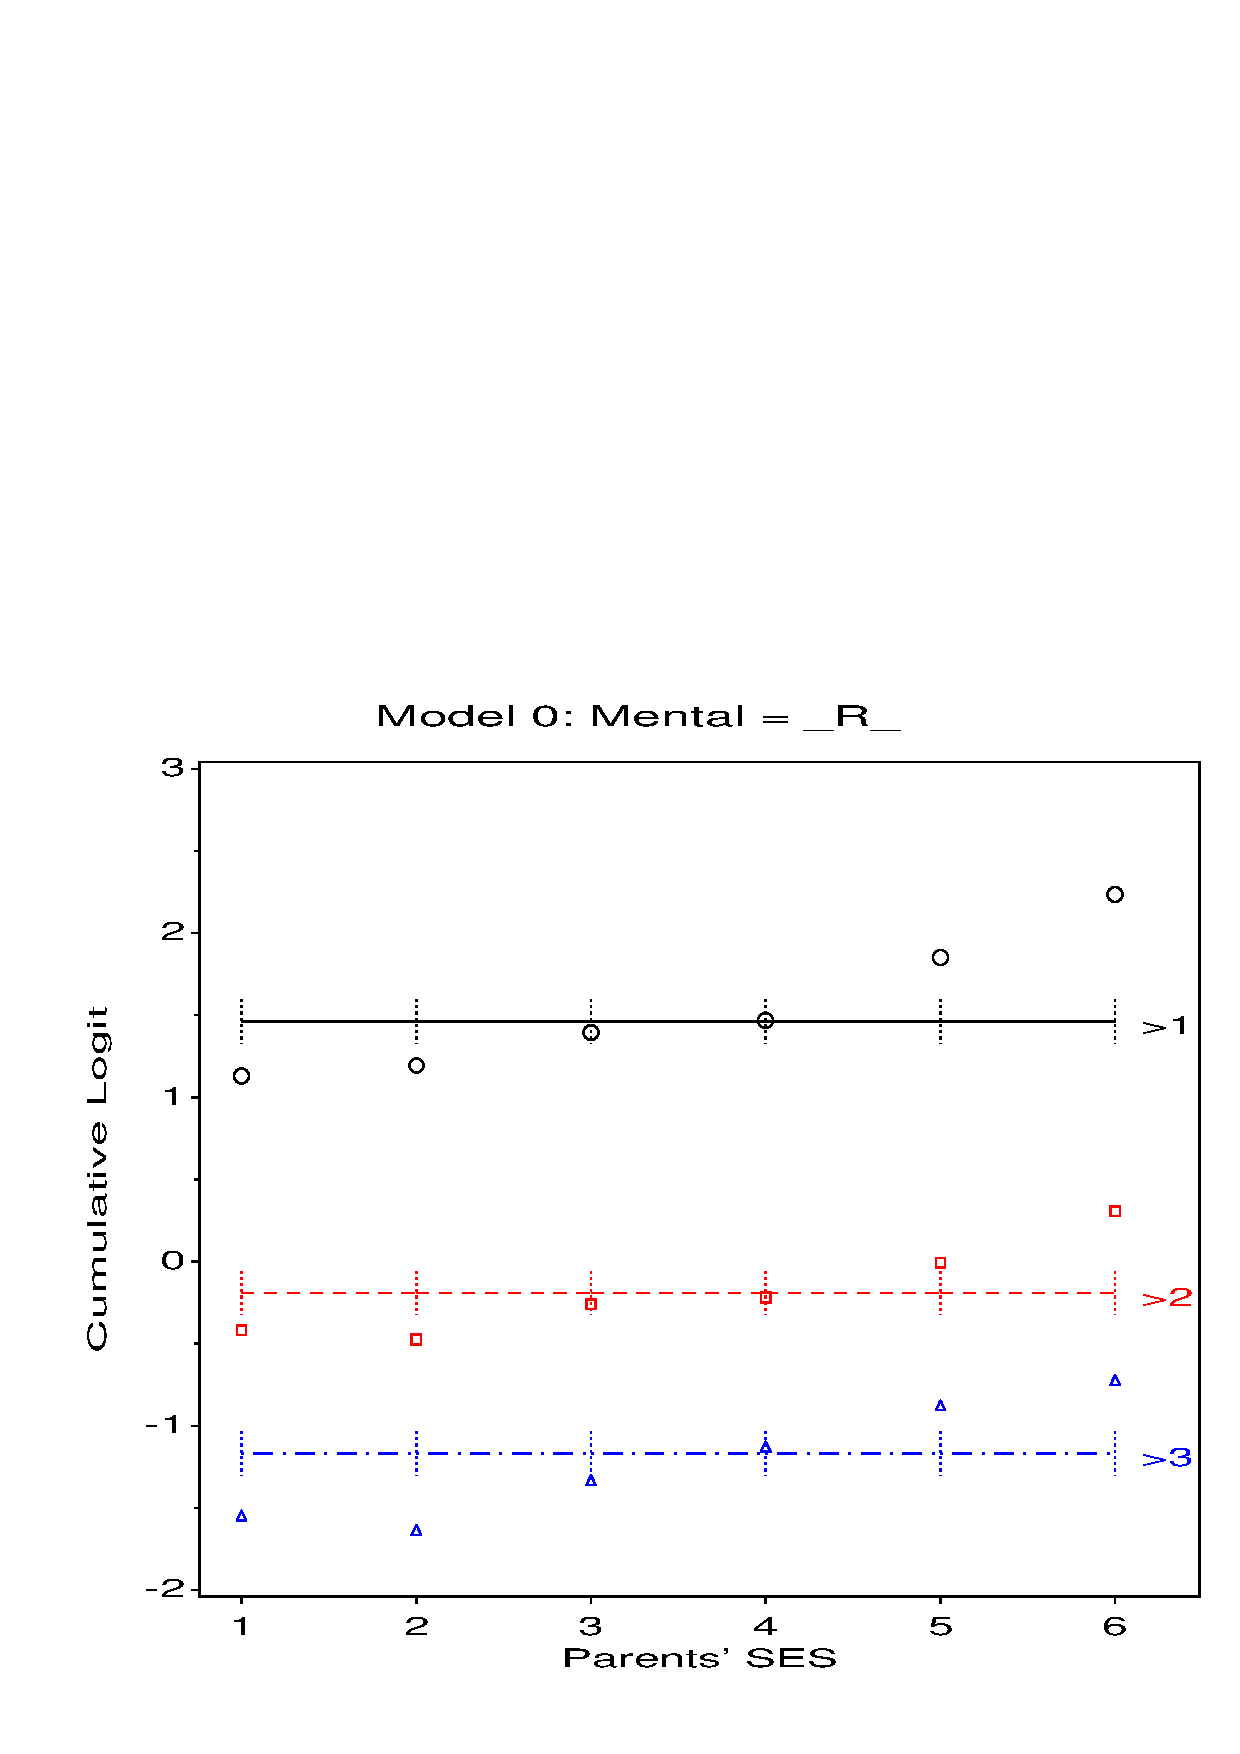
\includegraphics[width=1\linewidth]{mental31}
 \end{minipage}%
 \hfill
 \begin{minipage}[t]{.49\linewidth}
  \includegraphics[width=1\linewidth]{mental32}
 \end{minipage}
 \caption{Cumulative logit models for Mental Health data, Model 0 and Model 1}\label{fig:mental3a}
\end{figure}

%% two subfig side-by-side
\begin{figure}[htb]
 \begin{minipage}[t]{.49\linewidth}
  \includegraphics[width=1\linewidth]{mental33}
 \end{minipage}%
 \hfill
 \begin{minipage}[t]{.49\linewidth}
  \includegraphics[width=1\linewidth]{mental35}
 \end{minipage}
 \caption{Cumulative logit models for Mental Health data: Model 2 and Model 4}\label{fig:mental3b}
\end{figure}
\end{Example}

\subsection{Nested dichotomies}\label{sec:nested}

Nested dichotomies are successive binary partitions of the response
categories into nested sets.  For the levels of
a factor in an ANOVA design, nested dichotomies correspond to
orthogonal contrasts (assuming equal $n$s).

For example, the response categories
\{1,2,3,4\} could be divided first as \{1,2\} vs. \{3,4\}, as shown in the
left side of \figref{fig:nested}.  Then these two
dichotomies could be divided as \{1\} vs. \{2\}, and \{3\} vs. \{4\}.
Alternatively, these response categories could be divided as shown in the
right side of \figref{fig:nested}: first, \{1\} vs.
\{2,3,4\}, then \{2\} vs \{3,4\}, and finally \{3\} vs. \{4\}.  
\begin{figure}[htb]
  \centering
  \includegraphics[scale=.5]{ch6/fig/nested}
  \caption[Nested dichotomies]{Nested dichotomies.  The boxes show two different ways a four-category response can be represented as three nested dichotomies. Adapted from \citet{Fox:97}.}\label{fig:nested}
\end{figure}

Then,
\begin{itemize}

\item Each dichotomy can be fit using the familiar binary-response
 logistic model, and,
\item When the dichotomies are nested, the \(m - 1\) models will be statistically independent, so
that likelihood-ratio \(G^2\) statistics for overall fit, and
Wald statistics for individual terms will be additive.
\end{itemize}
Thus, we can treat the set of \(m - 1\) models as a single model
for the polytomous response, although we fit them separately for
computational purposes.  This approach to polytomous responses
is described in more detail by \citet{Fox:97}.

\begin{Example}[wlfpart]{Women's labor-force participation}
To illustrate, \citet{Fox:84,Fox:97} presented survey data on women's labor-force
participation in Canada in 1977.  Women were classified as not working
outside the home (n=155), working part-time (n=42)  or working
full-time (n=66).  Predictor variables were presence/absence of
children, and husband's income; a third variable, region of Canada,
is not considered here.  For these data, it makes sense to model the
log odds for two nested dichotomies:

\begin{itemize*}
\item Working vs. NotWorking
\item Working fulltime vs working parttime.
\end{itemize*}

The data are read in as shown below.
See \datref{dat:wlfdata} for the complete \Dset.  The 3-level variable
\pname{labor} is used to define two dichotomous variables, \pname{working}, and \pname{fulltime}.  Note that \pname{fulltime} is defined
(has non-missing values) only for working women.

\begin{listing}
proc format;
   value labor    /* labor-force participation */
      1 ='working full-time'  2 ='working part-time'
      3 ='not working';
   value kids     /* presence of children in the household */
      0 ='Children absent'  1 ='Children present';
data wlfpart;
   input case labor husinc children region;
   working = labor < 3;
   if working then
      fulltime = (labor = 1);
datalines;
  1  3  15  1  3
  2  3  13  1  3
  3  3  45  1  3
  4  3  23  1  3
  5  3  19  1  3
  {\it ... more data lines ...}
\end{listing}

An initial analysis attempts to fit the proportional odds model, with
the 3-level \pname{labor} variable as the response:

\begin{listing}
proc logistic data=wlfpart nosimple;
   {\bf model labor  = husinc children ;}
   title2 'Proportional Odds Model for Fulltime/Parttime/NotWorking';
\end{listing}

However, the proportional odds assumption is rejected by the score
test (see \outref{out:wlfpart.1}).

\begin{Output}[htb]
\caption{Test of the proportional odds assumption}\label{out:wlfpart.1}
\small
\begin{output}
          Score Test for the Proportional Odds Assumption

             Chi-Square = 18.5641 with 2 DF (p=0.0001)
\end{output}
\end{Output}

Hence, we fit models for each of the \pname{working} and \pname{fulltime}
dichotomies.  The \opt{descending}{LOGISTIC} is used so that in each
case the probability of a 1 response (working, or fulltime) will be
the event modeled.

\begin{listing}
proc logistic data=wlfpart nosimple descending;
   {\bf model working = husinc children ;}
   output out=resultw p=predict xbeta=logit;
   title2 'Nested Dichotomies';
run;
proc logistic data=wlfpart nosimple descending;
   {\bf model fulltime = husinc children ;}
   output out=resultf p=predict xbeta=logit;
\end{listing}

The \stmt{output}{LOGISTIC}s  create the \Dsets\ \pname{resultw} and
\pname{resultf} for plotting the predicted probabilities and logits.
The printed output for the working dichotomy is shown (partially)
in \outref{out:wlfpart.2}.

\begin{Output}[htb]
\caption{Women's labor-force data, analysis of the working/not working dichotomy}\label{out:wlfpart.2}
\small
\begin{output}
                               Response Profile
                          Ordered
                            Value  WORKING     Count

                                1        1       108
                                2        0       155

                  Testing Global Null Hypothesis: BETA=0
                            Intercept
               Intercept       and
   Criterion     Only      Covariates    Chi-Square for Covariates

   AIC           358.151      325.733      .
   SC            361.723      336.449      .
   -2 LOG L      356.151      319.733    36.418 with 2 DF (p=0.0001)
   Score            .            .       35.713 with 2 DF (p=0.0001)

                    Analysis of Maximum Likelihood Estimates

               Parameter Standard    Wald       Pr >    Standardized    Odds
   Variable DF  Estimate   Error  Chi-Square Chi-Square   Estimate     Ratio

   INTERCPT 1     1.3358   0.3838    12.1165     0.0005            .    .
   HUSINC   1    -0.0423   0.0198     4.5751     0.0324    -0.168541   0.959
   CHILDREN 1    -1.5756   0.2923    29.0651     0.0001    -0.398992   0.207
\end{output}
\end{Output}

To interpret the parameter estimates, note that the odds ratio of 0.959
for husband's income
means a 4\% decrease in the odds of working with each \$1000 increase in husband's income; an additional \$10,000 means a decrease in the odds
of working by
\(e^{-.423} = .655\).  Similarly, the effect of having children  corresponds
to an odds of working of .207 compared to those without children.

The output for the fulltime vs. parttime dichotomy is shown in
\outref{out:wlfpart.3}.
Note that nonworking women are excluded in this analysis.

\begin{Output}[htb]
\caption{Women's labor-force data, analysis of the fulltime/parttime dichotomy}\label{out:wlfpart.3}
\small
\begin{output}
                                Response Profile
                          Ordered
                            Value  FULLTIME     Count

                                1         1        66
                                2         0        42

   WARNING: 155 observation(s) were deleted due to missing values for
           the response or explanatory variables.

                   Testing Global Null Hypothesis: BETA=0
                             Intercept
                Intercept       and
   Criterion      Only      Covariates   Chi-Square for Covariates

   AIC            146.342      110.495      .
   SC             149.024      118.541      .
   -2 LOG L       144.342      104.495    39.847 with 2 DF (p=0.0001)
   Score             .            .       35.150 with 2 DF (p=0.0001)

                    Analysis of Maximum Likelihood Estimates

               Parameter Standard    Wald       Pr >    Standardized    Odds
   Variable DF  Estimate   Error  Chi-Square Chi-Square   Estimate     Ratio

   INTERCPT 1     3.4778   0.7671    20.5537     0.0001            .    .
   HUSINC   1    -0.1073   0.0392     7.5063     0.0061    -0.424867   0.898
   CHILDREN 1    -2.6515   0.5411    24.0135     0.0001    -0.734194   0.071
\end{output}
\end{Output}

Thus, the full 3-category response has been fitted by two models,

\begin{eqnarray}
  \log \left( \frac{ \Pr ( \mbox{working} ) }
  { \Pr ( \mbox{not working} ) } \right) & = &
  1.336 - 0.042 \,  \mbox{H\$} - 1.576 \,  \mbox{kids} \label{eq:wlfnest1}\\
%
  \log \left( \frac{ \Pr ( \mbox{fulltime} ) }
  { \Pr ( \mbox{parttime} ) } \right) & = &
  3.478 - 0.107 \,  \mbox{H\$} - 2.652 \,  \mbox{kids} \label{eq:wlfnest2}
\end{eqnarray}
The second equation gives the predicted log odds for
fulltime vs.\ parttime work {\it conditional} on working.

Because these models are nested, we can add the likelihood ratio or Wald tests across the
\ix{likelihood ratio test}
\ix{Wald test}
two models, so the overall test of the hypothesis that neither
husband's income nor presence of children predicts working status
(the 3-level response) has a \(G^2 = 36.42  +  39.85 = 66.27\) on
2+2=4 df (\(p < .0001\)).  Similarly, the hypothesis that husband's
income does not predict working status has a Wald-test \(G^2 = 4.58
+  7.51 = 12.09\) on 2 df (\(p < .001\)).

Comparison of the regression coefficients in the two sub-models (in
relation to the size of their standard errors) indicates why the
proportional odds model was not tenable.  The proportional odds model
requires that the coefficients for husband's income and children in
analogous models of the form \eqref{eq:logod1} and \eqref{eq:logod2}.
We can see that both variables have a
greater effect on the odds of fulltime vs. parttime work than on the
odds of working vs. not working.

As usual, these effects can be seen and interpreted more easily in a
graph (\figref{fig:wlfpart}).  The odds of working outside the home decrease as husband's
income increases and when there are children present.  However, among
working women, the odds of fulltime vs. parttime work decrease at a
faster rate with husband's income; women with children are less
likely to work fulltime.
\begin{figure}[htb]
  \centering
  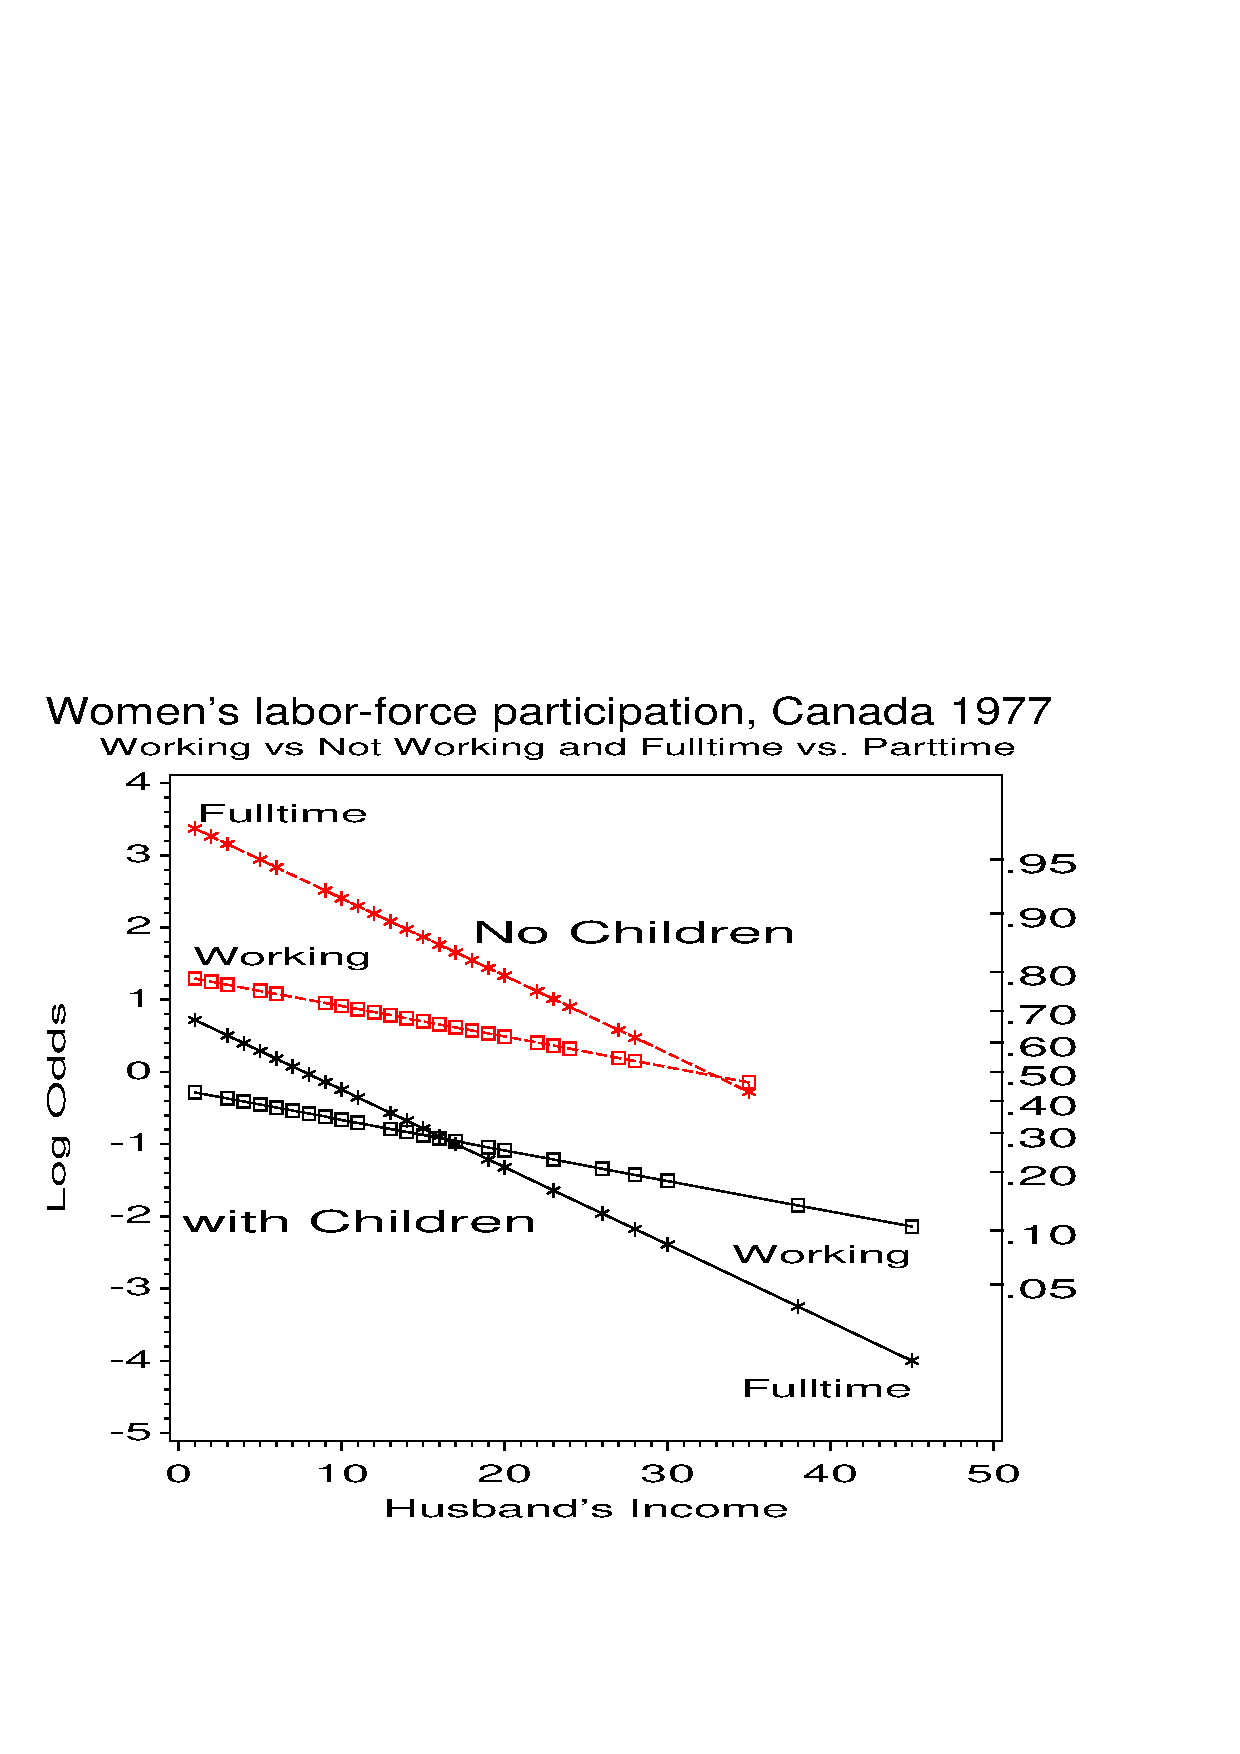
\includegraphics[scale=.7]{ch\thechapter/fig/wlfpart}
  \caption{Predicted log odds of working vs.\ not working, and of fulltime work vs.\ parttime work}\label{fig:wlfpart}
\end{figure}

To construct this graph, first join the separate results \Dsets\
into one.

\begin{listing}
*-- Merge the results to create one plot;
data both;
   set resultw(in=inw)
       resultf(in=inf);
   if inw then do;
      if children=1 then event='Working, with Children ';
      else event='Working, no Children ';
   end;
   else do;
      if children=1 then event='Fulltime, with Children ';
      else event='Fulltime, no Children ';
  end;
\end{listing}

Then, we can plot the log odds (or predicted probability) against
husband's income, using \pname{event} as to determine the curves to be
joined and labeled.
(The probability scale is constructed with the \macro{PSCALE}, and the
labels with an \ADS.  These steps are not similar to those described
in \exref{ex:arthrit10} and are
shown here).

\begin{listing}
proc gplot data=both;
   plot logit * husinc = event /
        anno=lbl nolegend frame vaxis=axis1;
   axis1 label=(a=90 'Log Odds') order=(-5 to 4);
   title2 'Working vs Not Working and Fulltime vs. Parttime';
   symbol1 v=dot    h=1.5 i=join l=3 c=red;
   symbol2 v=dot    h=1.5 i=join l=1 c=black;
   symbol3 v=circle h=1.5 i=join l=3 c=red;
   symbol4 v=circle h=1.5 i=join l=1 c=black;
\end{listing}
\end{Example}

\renewcommand{\FileName}{genlogit}
% slide template
\subsection{Basic ideas}
\begin{frame}
  \frametitle{Polytomous response: Generalized Logits}
  \begin{itemize}
	\item Models the probabilities of the $m$ response categories 
	as \(m - 1\) logits comparing
each of the first \(m - 1\) categories to the last (reference) category.
	\item Logits for any  pair of categories can be calculated
from the \(m - 1\) fitted ones.
	\item With $k$ predictors, \(x_1, x_2, \dots , x_k\), for $j=1, 2, \dots ,
	  m-1$, 
\begin{eqnarray*}
  L_{jm}  \equiv 
    \log \left( \frac{\pi_{ij}}{\pi_{im}} \right) & = & \beta_{0j}  +
  \beta _{1j} \,  x_{i1}  +
  \beta _{2j} \,  x_{i2}  + \cdots +
  \beta _{kj} \,  x_{ik} \quad \\
%  \mbox{for } j=1, 2, \dots , m-1 \\
  & = & \vec{\beta}_j \trans \vec{x}_i
\end{eqnarray*}

      \begin{itemize*}
	  \item One set of fitted coefficients, $\vec{\beta}_j$ for each
response category except the last.
	  \item Each coefficient, $\beta_{hj}$, gives the effect on the log odds
of a unit change in the predictor $x_h$
that an observation belongs to category $j$ vs.\ category $m$.
	  \end{itemize*}
	\item Probabilities in response caegories are calculated as:
\begin{equation*}
\pi_{ij} =
 \frac{ \exp ( \vec{\beta}_j \trans \vec{x}_i ) }
      { \sum_{j=1}^{m-1} \exp ( \vec{\beta}_j \trans \vec{x}_i ) }
	  \comma \, j=1,\dots, m-1 \,;
	  \quad\quad \pi_{im} = 1 - \sum_{j=1}^{m-1} \pi_{ij}
\end{equation*}
  \end{itemize}
\end{frame}

\begin{frame}[fragile]
  \frametitle{Polytomous response: Generalized Logits}
Fitting generalized logit models with SAS:
%  \begin{itemize}
%	\item SAS:
      \begin{itemize*}
	  \item Use \PROC{LOGISTIC} with \texttt{LINK=GLOGIT} option.
    	\begin{itemize*}
		\item \ODS\ $\rightarrow$ fitted probabilities, $\widehat{\pi}_{ij}$ for all $m$ categories
		\item Overall tests and specific tests for each predictor, for all $m$ categories
		\end{itemize*}
\vspace{2ex}
\begin{Input}[numbers=none]
proc logistic data=wlfpart;
   model labor = husinc children / \sasemph{link=glogit};
   output out=results p=predict xbeta=logit;
\end{Input}
	  \item Can also use \PROC{CATMOD} with \texttt{RESPONSE=LOGITS} statement.
    	\begin{itemize*}
		\item Same model, same predicted probabilities
		\item Different syntax, \ODS\ format, plotting steps
		\item Quantitative variables: \alert{\texttt{direct}} statement
		\end{itemize*}
\vspace{2ex}
\begin{Input}[numbers=none]
proc catmod data=wlfpart;
   \sasemph{direct husinc;}
   model labor = husinc children;
   \sasemph{response logits} / out=results;
\end{Input}
	  \end{itemize*} 

%  \end{itemize}
\end{frame}

\begin{frame}<1>[label=wlfpart5g]
  \frametitle{Example: Women's Labour Force Participation}
Graphs:
% two figures 
 \begin{minipage}[b]{.5\linewidth}
  \centering
  \includegraphics[width=.99\linewidth]{fig/wlfpart51}
 \end{minipage}%
 \begin{minipage}[b]{.5\linewidth}
  \centering
  \includegraphics[width=.99\linewidth]{fig/wlfpart52}
 \end{minipage}
\end{frame}


\begin{frame}[fragile]
  \frametitle{Example: Women's Labour Force Participation}
\begin{Input}[label=\fbox{\texttt{wlfpart5.sas} $\cdots$}]
title 'Generalized logit model';
proc logistic data=wlfpart;
   model labor = husinc children / \sasemph{link=glogit};
   \sasemph{output out=results p=predict xbeta=logit;}
\end{Input}
Response profile:
\begin{Output}[gobble=7]
                       Ordered                      Total
                         Value        labor     Frequency

                             1            1            66
                             2            2            42
                             3            3           155

             Logits modeled use labor=3 as the reference category.
\end{Output}
\emph{Note:} Not working is the baseline category
\end{frame}


\begin{frame}[fragile]
Overall and Type III tests:
\begin{Output}[gobble=7,baselinestretch=0.8]
                    Testing Global Null Hypothesis: BETA=0
 
            Test                 Chi-Square       DF     Pr > ChiSq

            Likelihood Ratio        77.6106        4         <.0001
            Score                   76.4850        4         <.0001
            Wald                    58.4351        4         <.0001

                          Type III Analysis of Effects
 
                                            Wald
                  Effect        DF    Chi-Square    Pr > ChiSq

                  husinc         2       12.8159        0.0016
                  children       2       53.9806        <.0001
\end{Output}
These are comparable to the combined tests for the nested dichotomies models.
\end{frame}

\begin{frame}[fragile]
Coefficients:
\begin{Output}[gobble=2,baselinestretch=0.8, fontsize=\footnotesize]
                    Analysis of Maximum Likelihood Estimates
 
                                          Standard          Wald
  Parameter    labor    DF    Estimate       Error    Chi-Square    Pr > ChiSq

  Intercept    1         1      1.9828      0.4842       16.7709        <.0001
  Intercept    2         1     -1.4323      0.5925        5.8445        0.0156
  husinc       1         1     -0.0972      0.0281       11.9762        0.0005
  husinc       2         1     0.00689      0.0235        0.0863        0.7689
  children     1         1     -2.5586      0.3622       49.9008        <.0001
  children     2         1      0.0215      0.4690        0.0021        0.9635
\end{Output}
i.e., the fitted models are:
\begin{eqnarray*}
  \log \left( \frac{ \Pr ( \mbox{fulltime} ) }
  { \Pr ( \mbox{not working} ) } \right) & = &
  1.983 - 0.097 \,  \mbox{H\$} - 2.56 \,  \mbox{kids} \\  %\label{eq:wlfgen1}
%
  \log \left( \frac{ \Pr ( \mbox{parttime} ) }
  { \Pr ( \mbox{not working} ) } \right) & = &
  -1.432 - 0.0069 \,  \mbox{H\$} - 0.0215 \,  \mbox{kids}  % \label{eq:wlfgen2}
\end{eqnarray*}
\emph{Interpretation:} Signs for \texttt{husinc} and \texttt{children} are understandable,
but need to make a plot!
\end{frame}

\begin{frame}[fragile]
\ODS\ \texttt{results} (for plots):
\begin{Output}[baselinestretch=0.7,gobble=2]
  case   labor   husinc  children   _LEVEL_     logit    predict

    1      3       15        1         1      -2.03423   0.09333
    1      3       15        1         2      -1.30743   0.19305
    1      3       15        1         3        .        0.71363
    2      3       13        1         1      -1.83977   0.11142
    2      3       13        1         2      -1.32122   0.18715
    2      3       13        1         3        .        0.70143
    3      3       45        1         1      -4.95114   0.00528
    3      3       45        1         2      -1.10067   0.24830
    3      3       45        1         3        .        0.74642
    4      3       23        1         1      -2.81207   0.04464
    4      3       23        1         2      -1.25230   0.21238
    4      3       23        1         3        .        0.74298
    5      3       19        1         1      -2.42315   0.06486
    5      3       19        1         2      -1.27987   0.20346
    5      3       19        1         3        .        0.73168
    6      3        7        1         1      -1.25639   0.18478
    6      3        7        1         2      -1.36257   0.16616
    ...
\end{Output}
\begin{itemize*}
	\item \texttt{logit} gives the two fitted log odds vs Not working
	\item \texttt{predict} gives the predicted probability for each category of \texttt{labor}
\end{itemize*}
\end{frame}

\begin{frame}[fragile]
  \frametitle{Example: Women's Labour Force Participation}
\begin{Input}[label=\fbox{$\cdots$ \texttt{wlfpart5.sas}},baselinestretch=0.7]
proc sort data=results;
   \sasemph{by children husinc _level_;}

   \sascomment{*-- Curve labels;}
%label(data=results, x=husinc, y=predict, cvar=_level_,
   by=children, subset=last._level_, text=put(_level_, labor.), 
   pos=2, out=labels1);

   \sascomment{*-- Panel labels;}
%label(data=results, x=20, y=0.85, 
   by=children, subset=last.children, text=put(children, kids.), 
   pos=2, size=2, out=labels2);
data labels;
   set labels1 labels2;
   by children;

goptions hby=0;
proc gplot data=results;
   \sasemph{plot predict * husinc = _level_} / 
      vaxis=axis1 hm=1 vm=1 \sasemph{anno=labels} nolegend;
   by children;
   axis1 order=(0 to .9 by .1) label=(a=90);
   symbol1 i=join v=circle   c=black;
   symbol2 i=join v=square   c=red;
   symbol3 i=join v=triangle c=blue;
   run;
\end{Input}
\end{frame}

\againframe<1>{wlfpart5g}
\endinput

% slide template
\begin{frame}
  \frametitle{}
  \begin{itemize}
	\item{\large\bfseries }
      \begin{itemize*}
	  \item 
    	\begin{itemize*}
		\item 
		\item 
		\end{itemize*}
	  \item 
	  \end{itemize*}
	\item{\large\bfseries }
	\item{\large\bfseries }
  \end{itemize}
\end{frame}


